% Created 2017-10-21 Sat 23:34
\documentclass[a4paper]{article}
\usepackage[utf8]{inputenc}
\usepackage[T1]{fontenc}
\usepackage{fixltx2e}
\usepackage{graphicx}
\usepackage{longtable}
\usepackage{float}
\usepackage{wrapfig}
\usepackage{rotating}
\usepackage[normalem]{ulem}
\usepackage{amsmath}
\usepackage{textcomp}
\usepackage{marvosym}
\usepackage{wasysym}
\usepackage{amssymb}
\usepackage{hyperref}
\tolerance=1000
\usepackage{minted}
\usepackage[margin=0.8in]{geometry}
\usepackage{amssymb,amsmath}
\usepackage{fancyhdr} %For headers and footers
\pagestyle{fancy} %For headers and footers
\usepackage{lastpage} %For getting page x of y
\usepackage{float} %Allows the figures to be positioned and formatted nicely
\restylefloat{figure} %and this command
\usepackage{hyperref}
\hypersetup{urlcolor=blue}
\usepackage{minted}
\setminted{frame=single,framesep=10pt}
\chead{}
\rhead{\today}
\cfoot{}
\rfoot{\thepage\ of \pageref{LastPage}}
\usepackage[parfill]{parskip}
\usepackage{subfig}
\hypersetup{colorlinks=true,linkcolor=black}
\AtBeginEnvironment{minted}{%
\renewcommand{\fcolorbox}[4][]{#4}}
\usepackage{framed}
\author{Nathan Hughes (\href{mailto:nah31@aber.ac.uk}{nah26@aber.ac.uk})}
\date{\today}
\title{Assignment 1}
\hypersetup{
  pdfkeywords={},
  pdfsubject={},
  pdfcreator={Emacs 25.3.1 (Org mode 8.2.10)}}
\begin{document}

\maketitle
\vspace{2cm}

\begin{center}

\includegraphics[width=4cm]{./ruby.png}
\end{center}

\clearpage
\tableofcontents
\clearpage


\section{Introduction}
\label{sec-1}

\section{CSA Architecture}
\label{sec-2}

\subsection{User creation}
\label{sec-2-1}

\subsection{Post creation}
\label{sec-2-2}

\subsection{Routes}
\label{sec-2-3}
\begin{listing}[H]
\begin{minted}[]{ruby}
Rails.application.routes.draw do
  resources :users
  resources :posts
  # For details on the DSL available within this file, see http://guides.rubyonrails.org/routing.html

  root 'posts#index'
  # Send errors to root
  get '*path' => redirect('/')

end
\end{minted}
\caption{x}
\end{listing}

\subsection{Navigation}
\label{sec-2-4}
\begin{listing}[H]
\begin{minted}[]{ruby}
primary.item :home, 'Home', '/home', highlights_on: /(^\/$)|(^\/home$)/
primary.item :jobs, 'Jobs', '/jobs'
primary.item :profile, 'Profile', '/profile', if: Proc.new { is_admin? }
primary.item :users, 'Users', users_path, if: Proc.new { is_admin? }
primary.item :broadcasts, 'Broadcasts', '/broadcasts', if: Proc.new { is_admin? }
\end{minted}
\caption{x}
\end{listing}

\subsection{Application Controller}
\label{sec-2-5}
\begin{listing}[H]
\begin{minted}[]{ruby}
# Make is_admin? a helper method available to view templates
helper_method :is_admin?

protected

# Is the caller an admin user? Currently everyone is!
# @return true if admin user else false
def is_admin?
  true
end
\end{minted}
\caption{x}
\end{listing}

\subsection{Layout.scss}
\label{sec-2-6}

\begin{minted}[]{css}
.navigation {

  a {
    color: #aa1111;
    text-decoration: none;
    font-weight: bold;
    margin: 0;
    padding-left: 0.5em;
    padding-right: 0.5em;
  }

  .selected {
    background-color: #C5F1F9;
  }

  a:hover,
  a:active,
  a.here:link,
  a.here:visited {
    color: #C811D8;
  }
\end{minted}



\section{{\bfseries\sffamily TODO} MVC Model}
\label{sec-3}

\subsection{{\bfseries\sffamily TODO} UML Diagram}
\label{sec-3-1}
\subsubsection{Database}
\label{sec-3-1-1}
\begin{center}
\begin{figure}[htb]
\centering
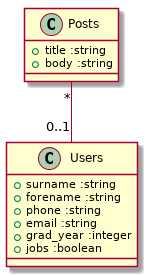
\includegraphics[width=4cm]{posts-users.png}
\caption{Posts and Users UML}
\end{figure}
\end{center}

\subsubsection{{\bfseries\sffamily TODO} What is the Model-2 Variant}
\label{sec-3-1-2}
\subsection{{\bfseries\sffamily TODO} Models}
\label{sec-3-2}
\subsection{{\bfseries\sffamily TODO} Views}
\label{sec-3-3}
\subsection{{\bfseries\sffamily TODO} Controls}
\label{sec-3-4}


\section{Database}
\label{sec-4}

\subsection{{\bfseries\sffamily TODO} Database location}
\label{sec-4-1}

\subsection{{\bfseries\sffamily TODO} Migration Files}
\label{sec-4-2}
\begin{minted}[]{bash}
rails db:migrate
\end{minted}
% Emacs 25.3.1 (Org mode 8.2.10)
\end{document}